\documentclass[]{article}
\usepackage{lmodern}
\usepackage{amssymb,amsmath}
\usepackage{ifxetex,ifluatex}
\usepackage{fixltx2e} % provides \textsubscript
\ifnum 0\ifxetex 1\fi\ifluatex 1\fi=0 % if pdftex
  \usepackage[T1]{fontenc}
  \usepackage[utf8]{inputenc}
\else % if luatex or xelatex
  \ifxetex
    \usepackage{mathspec}
  \else
    \usepackage{fontspec}
  \fi
  \defaultfontfeatures{Ligatures=TeX,Scale=MatchLowercase}
\fi
% use upquote if available, for straight quotes in verbatim environments
\IfFileExists{upquote.sty}{\usepackage{upquote}}{}
% use microtype if available
\IfFileExists{microtype.sty}{%
\usepackage{microtype}
\UseMicrotypeSet[protrusion]{basicmath} % disable protrusion for tt fonts
}{}
\usepackage[margin=1in]{geometry}
\usepackage{hyperref}
\hypersetup{unicode=true,
            pdftitle={HW 5},
            pdfauthor={Olga Lyashevskaya, George Moroz, Alla Tambovtseva and Ilya Schurov},
            pdfborder={0 0 0},
            breaklinks=true}
\urlstyle{same}  % don't use monospace font for urls
\usepackage{graphicx,grffile}
\makeatletter
\def\maxwidth{\ifdim\Gin@nat@width>\linewidth\linewidth\else\Gin@nat@width\fi}
\def\maxheight{\ifdim\Gin@nat@height>\textheight\textheight\else\Gin@nat@height\fi}
\makeatother
% Scale images if necessary, so that they will not overflow the page
% margins by default, and it is still possible to overwrite the defaults
% using explicit options in \includegraphics[width, height, ...]{}
\setkeys{Gin}{width=\maxwidth,height=\maxheight,keepaspectratio}
\IfFileExists{parskip.sty}{%
\usepackage{parskip}
}{% else
\setlength{\parindent}{0pt}
\setlength{\parskip}{6pt plus 2pt minus 1pt}
}
\setlength{\emergencystretch}{3em}  % prevent overfull lines
\providecommand{\tightlist}{%
  \setlength{\itemsep}{0pt}\setlength{\parskip}{0pt}}
\setcounter{secnumdepth}{0}
% Redefines (sub)paragraphs to behave more like sections
\ifx\paragraph\undefined\else
\let\oldparagraph\paragraph
\renewcommand{\paragraph}[1]{\oldparagraph{#1}\mbox{}}
\fi
\ifx\subparagraph\undefined\else
\let\oldsubparagraph\subparagraph
\renewcommand{\subparagraph}[1]{\oldsubparagraph{#1}\mbox{}}
\fi

%%% Use protect on footnotes to avoid problems with footnotes in titles
\let\rmarkdownfootnote\footnote%
\def\footnote{\protect\rmarkdownfootnote}

%%% Change title format to be more compact
\usepackage{titling}

% Create subtitle command for use in maketitle
\newcommand{\subtitle}[1]{
  \posttitle{
    \begin{center}\large#1\end{center}
    }
}

\setlength{\droptitle}{-2em}

  \title{HW 5}
    \pretitle{\vspace{\droptitle}\centering\huge}
  \posttitle{\par}
    \author{Olga Lyashevskaya, George Moroz, Alla Tambovtseva and Ilya Schurov}
    \preauthor{\centering\large\emph}
  \postauthor{\par}
    \date{}
    \predate{}\postdate{}
  

\begin{document}
\maketitle

\subsection{HW for theoretical
linguists}\label{hw-for-theoretical-linguists}

There are several tasks on

\begin{itemize}
\tightlist
\item
  data manipulation with \texttt{dplyr} (if you have any problems see
  \href{https://www.datacamp.com/courses/dplyr-data-manipulation-r-tutorial}{this}
  and
  \href{https://www.datacamp.com/courses/joining-data-in-r-with-dplyr}{this}
  courses)
\item
  data visualisation with \texttt{ggplot2} (if you have any problems see
  \href{https://www.datacamp.com/courses/data-visualization-with-ggplot2-1}{this
  course})
\end{itemize}

\subsubsection{1.}\label{section}

These datasets contains the results of the experiment that evaluates the
inter speaker variation in noun class assignment among speakers of the
Zilo dialect of Andi (a Nakh-Daghestanian language spoken in the
Republic of Daghestan). In Zilo there are two classes for inanimate
objects with no obvious semantic distinction between them.

There are two datasets:

\begin{itemize}
\tightlist
\item
  zilo\_class\_experiment\_data.csv
\item
  w\_id --- word id
\item
  stimulus --- stimuli word in Zilo
\item
  translation\_en --- translation to English
\item
  stimulus\_source --- the source of the stimulus: native or loan
\item
  1 \ldots{} 16 --- columns that contain answers of 16 speakers of Zilo:
  \texttt{b} or \texttt{r} (class markers)
\item
  zilo\_class\_experiment\_informants.csv
\item
  s\_id --- speaker id (corresponds to numbers in the previous dataset)
\item
  sex --- sex of the speaker
\item
  age\_2017 --- age of the speaker on the moment of the interview
\end{itemize}

Calculate the ratio of b-words
(\(\frac{b\text{-words}}{b\text{-words}+r\text{-words}}\)) for each sex
and stimulus source and visualise it with the following graph (it is
possible to do within one pipe).

\begin{verbatim}
## Parsed with column specification:
## cols(
##   .default = col_character(),
##   w_id = col_double()
## )
\end{verbatim}

\begin{verbatim}
## See spec(...) for full column specifications.
\end{verbatim}

\begin{verbatim}
## Parsed with column specification:
## cols(
##   s_id = col_double(),
##   sex = col_character(),
##   age_2017 = col_double()
## )
\end{verbatim}

\begin{verbatim}
## Joining, by = "s_id"
\end{verbatim}

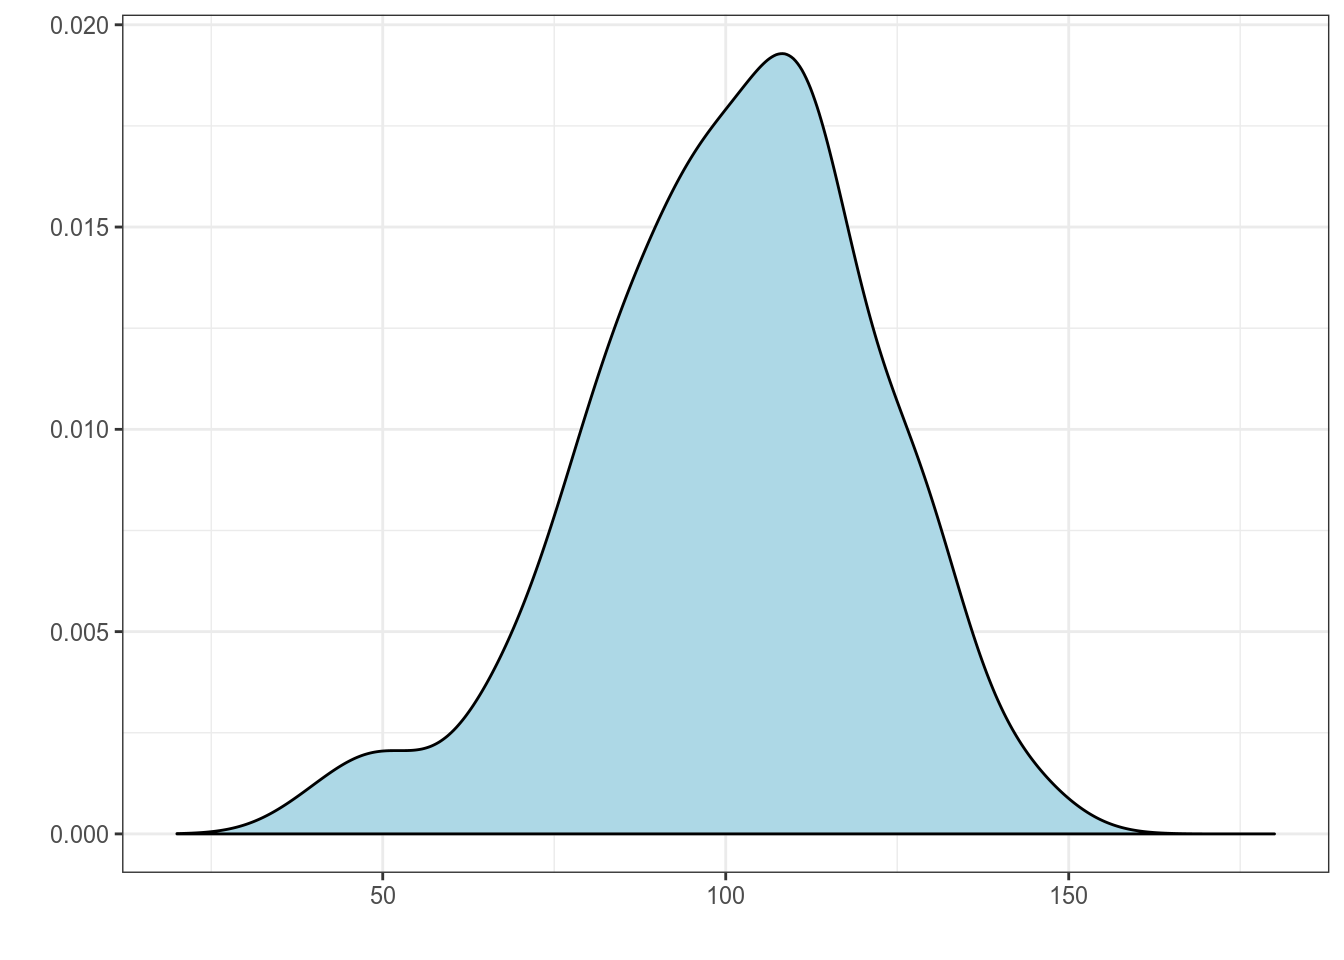
\includegraphics{LingData-HW6_files/figure-latex/unnamed-chunk-1-1.pdf}

\subsection{HW for computer linguists}\label{hw-for-computer-linguists}

There are several tasks on

\begin{itemize}
\tightlist
\item
  data manipulation with \texttt{dplyr} (if you have any problems see
  \href{https://www.datacamp.com/courses/dplyr-data-manipulation-r-tutorial}{this}
  and
  \href{https://www.datacamp.com/courses/joining-data-in-r-with-dplyr}{this}
  courses)
\item
  data visualisation with \texttt{ggplot2} (if you have any problems see
  \href{https://www.datacamp.com/courses/data-visualization-with-ggplot2-1}{this
  course})
\end{itemize}


\end{document}
